\documentclass[a4paper,14pt,oneside,final]{extarticle}
\usepackage[top=2cm, bottom=2cm, left=3cm, right=1cm]{geometry}
\usepackage{scrextend}

\usepackage[T2A,T1]{fontenc}
\usepackage[ukrainian,russian,english]{babel}
\usepackage{tempora}
\usepackage{fontspec}
\setmainfont{tempora}

% Зачем: Отключает использование изменяемых межсловных пробелов.
% Почему: Так не принято делать в текстах на русском языке.
\frenchspacing

\usepackage{indentfirst}
\setlength{\parindent}{1.25cm}
\renewcommand{\baselinestretch}{1.5}

% Header
\usepackage{fancyhdr}
\pagestyle{fancy}
\fancyhead{}
\fancyfoot{}
\fancyhead[R]{\small \selectfont \thepage}
\renewcommand{\headrulewidth}{0pt}

% Captions
\usepackage{chngcntr}
\counterwithin{figure}{section}
\counterwithin{table}{section}
\usepackage[tableposition=top]{caption}
\usepackage{subcaption}
\DeclareCaptionLabelFormat{gostfigure}{Рисунок #2}
\DeclareCaptionLabelFormat{gosttable}{Таблиця #2}
\DeclareCaptionLabelSeparator{gost}{~---~}
\captionsetup{labelsep=gost}
\captionsetup[figure]{labelformat=gostfigure}
\captionsetup[table]{labelformat=gosttable}
\renewcommand{\thesubfigure}{\asbuk{subfigure}}

% Sections
\usepackage[explicit]{titlesec}
\newcommand{\sectionbreak}{\clearpage}

\titleformat{\section}
  {\centering}{\thesection \quad}{0pt}{\MakeUppercase{#1}}
\titleformat{\subsection}[block]
  {\bfseries}{\thesubsection \quad #1}{0cm}{}

\titlespacing{\section} {0cm}{0cm}{21pt}
\titlespacing{\subsection} {\parindent}{21pt}{0cm}
\titlespacing{\subsubsection} {\parindent}{0cm}{0cm}

% Lists
\usepackage{enumitem}
\renewcommand\labelitemi{--}
\setlist[itemize]{noitemsep, topsep=0pt, wide}
\setlist[enumerate]{noitemsep, topsep=0pt, wide, label=\arabic*}
\setlist[description]{labelsep=0pt, noitemsep, topsep=0pt, leftmargin=2\parindent, labelindent=\parindent, labelwidth=\parindent, font=\normalfont}

% Toc
\usepackage{tocloft}
\tocloftpagestyle{fancy}
\renewcommand{\cfttoctitlefont}{}
\setlength{\cftbeforesecskip}{0pt}
\renewcommand{\cftsecfont}{}
\renewcommand{\cftsecpagefont}{}
\renewcommand{\cftsecleader}{\cftdotfill{\cftdotsep}}

\usepackage{float}
\usepackage{pgfplots}
\usepackage{graphicx}
\usepackage{multirow}
\usepackage{amssymb,amsfonts,amsmath,amsthm}
\usepackage{csquotes}

\usepackage{listings}
\lstset{basicstyle=\footnotesize\ttfamily,breaklines=true}
\lstset{language=Matlab}

\usepackage[
	backend=biber,
	sorting=none,
	language=auto,
	autolang=other
]{biblatex}
\DeclareFieldFormat{labelnumberwidth}{#1}


\newcommand{\labnumber}{4} % fourth lab
\documentclass[a4paper,14pt,oneside,final]{extarticle}
\usepackage[top=2cm, bottom=2cm, left=3cm, right=1cm]{geometry}
\usepackage{scrextend}

\usepackage[T2A,T1]{fontenc}
\usepackage[ukrainian,russian,english]{babel}
\usepackage{tempora}
\usepackage{fontspec}
\setmainfont{tempora}

% Зачем: Отключает использование изменяемых межсловных пробелов.
% Почему: Так не принято делать в текстах на русском языке.
\frenchspacing

\usepackage{indentfirst}
\setlength{\parindent}{1.25cm}
\renewcommand{\baselinestretch}{1.5}

% Header
\usepackage{fancyhdr}
\pagestyle{fancy}
\fancyhead{}
\fancyfoot{}
\fancyhead[R]{\small \selectfont \thepage}
\renewcommand{\headrulewidth}{0pt}

% Captions
\usepackage{chngcntr}
\counterwithin{figure}{section}
\counterwithin{table}{section}
\usepackage[tableposition=top]{caption}
\usepackage{subcaption}
\DeclareCaptionLabelFormat{gostfigure}{Рисунок #2}
\DeclareCaptionLabelFormat{gosttable}{Таблиця #2}
\DeclareCaptionLabelSeparator{gost}{~---~}
\captionsetup{labelsep=gost}
\captionsetup[figure]{labelformat=gostfigure}
\captionsetup[table]{labelformat=gosttable}
\renewcommand{\thesubfigure}{\asbuk{subfigure}}

% Sections
\usepackage[explicit]{titlesec}
\newcommand{\sectionbreak}{\clearpage}

\titleformat{\section}
  {\centering}{\thesection \quad}{0pt}{\MakeUppercase{#1}}
\titleformat{\subsection}[block]
  {\bfseries}{\thesubsection \quad #1}{0cm}{}

\titlespacing{\section} {0cm}{0cm}{21pt}
\titlespacing{\subsection} {\parindent}{21pt}{0cm}
\titlespacing{\subsubsection} {\parindent}{0cm}{0cm}

% Lists
\usepackage{enumitem}
\renewcommand\labelitemi{--}
\setlist[itemize]{noitemsep, topsep=0pt, wide}
\setlist[enumerate]{noitemsep, topsep=0pt, wide, label=\arabic*}
\setlist[description]{labelsep=0pt, noitemsep, topsep=0pt, leftmargin=2\parindent, labelindent=\parindent, labelwidth=\parindent, font=\normalfont}

% Toc
\usepackage{tocloft}
\tocloftpagestyle{fancy}
\renewcommand{\cfttoctitlefont}{}
\setlength{\cftbeforesecskip}{0pt}
\renewcommand{\cftsecfont}{}
\renewcommand{\cftsecpagefont}{}
\renewcommand{\cftsecleader}{\cftdotfill{\cftdotsep}}

\newcommand{\khpistudentgroup}{КН-34г}
\newcommand{\khpistudentname}{Чепурний~А.~С.}

\newcommand{\khpidepartment}{Програмна інженерія та інформаційні технології управління}
\newcommand{\khpititlewhat}{
	Лабораторна робота №\labnumber \\
	з предмету <<Моделювання систем>>
}
\newcommand{\khpititlewho}{
	Виконав: \\
	\hspace*{\parindent} ст. групи \khpistudentgroup \\
	\hspace*{\parindent} \khpistudentname \\
	Перевірила: \\
	\hspace*{\parindent} ст. в. каф. ПІІТУ \\
	\hspace*{\parindent} Єршова~С.~І. \\
	\hspace*{\parindent} ас. каф. ПІІТУ \\
	\hspace*{\parindent} Литвинова~Ю.~С. \\
}



\usepackage{systeme}
\usepackage{longtable,tabu}
\usepackage{multirow}
\usepackage{array,multirow}
\usepackage{pdflscape}
\usepackage{afterpage}
\usepackage{bm}

\begin{document}
\Ukrainian

\begin{titlepage}

\begin{center}
	МІНІСТЕРСТВО ОСВІТИ І НАУКИ УКРАЇНИ \\
	НАЦІОНАЛЬНИЙ ТЕХНІЧНИЙ УНІВЕРСИТЕТ \\
	«ХАРКІВСЬКИЙ ПОЛІТЕХНІЧНИЙ ІНСТИТУТ» \\[0.5cm]
	Кафедра <<\khpidepartment>> \\
\end{center}

\vspace{6cm}

\begin{center}
	\khpititlewhat
\end{center}

\vspace{3cm}

\begin{addmargin}[10cm]{0cm}
	\khpititlewho
\end{addmargin}

\vspace{\fill}

\begin{center}
	Харків \the\year
\end{center}

\end{titlepage}

\addtocounter{page}{1}

\textbf{Тема роботи}: Рішення багатокритеріальної задачі лінійного програмування методом обмежень.

\textbf{Завдання для виконання}
\begin{itemize}
	\item вирішити таку багатокритеріальну задачу лінійного програмування методом обмежень одним способом, описаним в прикладі;
	\item для кожного рішення подати такі результати:
	\begin{enumerate}[label=\arabic*)]
		\item чисельне значення вектора вагових коефіцієнтів;
		\item чисельні значення перетворених критеріїв;
		\item добутку вектора вагових коефіцієнтів на відповідні чисельні значення перетворених критеріїв;
		\item чисельні значення змінних, в тому числі додатково введеної змінної;
		\item чисельні значення цільових функцій;
	\end{enumerate}
	\item порівняти отримані результати з результатами, отриманими за допомогою теорем: Карліна, Гермейера і третьої теореми по знаходженню ефективних альтернатив (з відповідними значеннями вектора вагових коефіцієнтів), провести аналіз отриманих результатів.
\end{itemize}

Вариант №1

\begin{align*}
k_{u_1}=0.68, k_{u_2}=0.83.
\end{align*}

{
	\small
	\tabulinesep=1.2mm
	\begin{longtabu} to \textwidth {|X[12,l]|X[1,c]X[1,c]X[1,c]|X[1,c]X[1,c]X[1,c]|X[1,c]X[1,c]X[1,c]|X[1,c]X[1,c]X[1,c]|X[1,c]X[1,c]X[1,c]|}  
		\caption{Самооценка экспертов}
		\label{tab:selfscore} \\
		\hline
		\multirow{3}{*}{Источник аргументации} & \multicolumn{15}{c|}{Уровень влияния источника на мнение эксперта} \\ \cline{2-16}
		& \multicolumn{3}{c|}{Эксперт 1} & \multicolumn{3}{c|}{Эксперт 2} & \multicolumn{3}{c|}{Эксперт 3} & \multicolumn{3}{c|}{Эксперт 4} & \multicolumn{3}{c|}{Эксперт 5} \\ \cline{2-16}
		& A & B & C & A & B & C & A & B & C & A & B & C & A & B & C \\ \hline
		\endfirsthead

		\caption*{Окончание таблицы \thetable{}}\\
	    \hline
		\multirow{3}{*}{Источник аргументации} & \multicolumn{15}{c|}{Уровень влияния источника на мнение эксперта} \\ \cline{2-16}
		& \multicolumn{3}{c|}{Эксперт 1} & \multicolumn{3}{c|}{Эксперт 2} & \multicolumn{3}{c|}{Эксперт 3} & \multicolumn{3}{c|}{Эксперт 4} & \multicolumn{3}{c|}{Эксперт 5} \\ \cline{2-16}
		& A & B & C & A & B & C & A & B & C & A & B & C & A & B & C \\ \hline
		\endhead

	 	Проведенный экспертом теоретический анализ данной проблемы 
		& & \checkmark & & & \checkmark & & & \checkmark & & \checkmark & & & & & \checkmark \\ \hline
		Производственный опыт эксперта, связанный с решаемой проблемой & \checkmark & & & & \checkmark & & & \checkmark & & & \checkmark & & & & \checkmark \\ \hline
		Участие в семинарах, совещаниях в своей стране по исследуемой проблеме & & & \checkmark & & & \checkmark & \checkmark & & & & \checkmark & & & \checkmark & \\ \hline
		Знакомство с работами зарубежных авторов по рассматриваемой проблеме & & & \checkmark & & & \checkmark & \checkmark & & & & & \checkmark & & \checkmark & \\ \hline
		Количество проектов, в подготовке, реализации и экспертизе которых эксперт принимал участие & & \checkmark & & & \checkmark & & & \checkmark & & \checkmark & & & & & \checkmark \\ \hline
		Влияние интуиции эксперта на принимаемые решения & & \checkmark & & \checkmark & & & & \checkmark & & & \checkmark & & \checkmark & & \\ \hline
	\end{longtabu}
}

{
	\small
	\tabulinesep=1.2mm
	\begin{longtabu} to \textwidth {|X[1,c]|X[1,c]|X[1,c]|X[1,c]|X[1,c]|X[1,c]|X[1,c]|}  
		\caption{Параметры экспертов}
		\label{tab:score} \\
		\hline
		$k_i$  & $u$ & Эксперт 1 & Эксперт 2 & Эксперт 3 & Эксперт 4 & Эксперт 5 \\ \hline
		\endfirsthead

		\caption*{Окончание таблицы \thetable{}}\\
	    \hline
		$k_i$  & $u$ & Эксперт 1 & Эксперт 2 & Эксперт 3 & Эксперт 4 & Эксперт 5 \\ \hline
		\endhead

	 	$0.0003$ & $u_{lt} $ & $34$ & $26$ & $52$ & $41$ & $60$ \\ \hline
	 	$0.0008$ & $u_{sm} $ & $2$ & $14$ & $15$ & $3$ & $16$ \\ \hline
	 	$0.0015$ & $u_{sd} $ & $16$ & $3$ & $20$ & $21$ & $12$ \\ \hline
	 	$0.0020$ & $u_{z3} $ & $12$ & $14$ & $2$ & $2$ & $32$ \\ \hline
	 	$0.0010$ & $u_{z5} $ & $16$ & $23$ & $24$ & $10$ & $39$ \\ \hline
	 	$0.0009$ & $u_{zsp} $ & $5$ & $2$ & $14$ & $8$ & $9$ \\ \hline
	 	$0.0010$ & $u_{zv} $ & $26$ & $7$ & $2$ & $20$ & $32$ \\ \hline
	 	$0.0015$ & $u_{vs} $ & $5$ & $12$ & $5$ & $2$ & $3$ \\ \hline
	 	$0.0020$ & $u_{vz} $ & $1$ & $2$ & $4$ & $7$ & $0$ \\ \hline
	 	$0.0033$ & $u_{vsp} $ & $18$ & $23$ & $7$ & $21$ & $5$ \\ \hline
	 	$0.0080$ & $u_{zdl} $ & $4$ & $3$ & $5$ & $5$ & $4$ \\ \hline
	 	$0.0070$ & $u_{dlz} $ & $4$ & $3$ & $4$ & $4$ & $4$ \\ \hline
	 	$0.0015$ & $u_{kn} $ & $1$ & $1$ & $1$ & $1$ & $1$ \\ \hline
	 	$0.0200$ & $u_{dn} $ & $0$ & $0$ & $1$ & $1$ & $1$ \\ \hline
	 	$0.0250$ & $u_{zd} $ & $1$ & $0$ & $1$ & $1$ & $1$ \\ \hline
	 	$0.0300$ & $u_{zn} $ & $1$ & $1$ & $1$ & $1$ & $1$ \\ \hline
	 	$0.0350$ & $u_{zpf} $ & $0$ & $0$ & $1$ & $0$ & $1$ \\ \hline
	 	$0.0015$ & $u_{pv} $ & $6$ & $4$ & $15$ & $3$ & $13$ \\ \hline
	 	$0.0018$ & $u_{pn} $ & $2$ & $4$ & $0$ & $6$ & $2$ \\ \hline
	 	$0.0020$ & $u_{ps} $ & $1$ & $0$ & $3$ & $2$ & $8$ \\ \hline
		$0.0250$ & $u_{sk} $ & $0.7$ & $0.65$ & $0.87$ & $0.93$ & $0.84$ \\ \hline
	 	$0.0015$ & $u_{skp} $ & $0.83$ & $0.84$ & $0.79$ & $0.85$ & $0.91$ \\ \hline
	 	$-0.0005$ & $u_{usn} $ & $0$ & $0$ & $0$ & $0$ & $0$ \\ \hline
	 	$0.0003$ & $u_{usi} $ & $0$ & $0$ & $0$ & $0$ & $0$ \\ \hline
	 	$0.0010$ & $u_{usj} $ & $0$ & $0$ & $0$ & $1$ & $0$ \\ \hline
	 	$0.0380$ & $u_{usv} $ & $1$ & $1$ & $1$ & $0$ & $1$ \\ \hline
	 	$0.0100$ & $u_{izp} $ & $5$ & $4$ & $5$ & $5$ & $4$ \\ \hline
	 	$0.0086$ & $u_{ikr} $ & $4$ & $5$ & $5$ & $5$ & $4$ \\ \hline
	 	$-0.0015$ & $u_{iuk} $ & $1$ & $1$ & $2$ & $1$ & $1$ \\ \hline
	 	$0.0100$ & $u_{ilz} $ & $1$ & $0$ & $0$ & $1$ & $1$ \\ \hline
	 	$0.0080$ & $u_{iak} $ & $5$ & $4$ & $3$ & $5$ & $5$ \\ \hline
	\end{longtabu}
}


\subsection{Формування багатокритерільної задачі лінійного програмування}

З використанням раніш визначеної багатокритеріальної задачі в загальному вигляді сформуємо багатокритеріальну задачу, що належить до класу задач лінійного програмування. 
У цьому випадку особливістю багатокритеріальної задачі буде вимога про дотримання властивості лінійності для множини функцій мети $\{ f_i(\vec{x}), i \in I \}$ та множини функцій $\{ \phi_j(\vec{x}), j \in J\}$, які визначають обмеження задачі.

З урахуванням вищевикладеного формально багатокритеріальна задача лінійного програмування може бути подана в наступному вигляді:
\begin{gather*}
	f_i(x) = \sum_{l \in L}{c_l^i x_l} \to \max, i \in I_1, \\
	f_i(x) = \sum_{l \in L}{c_l^i x_l} \to \min, i \in I_2, \\
	\sum_{l \in L}{a_{jl} x_l \quad * \quad b_j}, j \in J,
\end{gather*}
\begin{description}
	\item[де] $* \in \{$\leq$, $\geq$, $=$\}$.
\end{description}

Для розв'язання цієї задачі застосуємо метод обмежень. 
Відповідно до методу обмежень необхідно провести перетворення вихідної множини функцій мети до безрозмірного вигляду одним із припустимих варіантів:
\begin{equation}\label{eq:omega}
\omega^1_i(f_i(\vec{x})) = \systeme[][:]{
\cfrac{f_i^0-f_i(\vec{x})}{f_i^0 - f_{i(\min)}},i \in I_1
:
\cfrac{f_i(\vec{x})-f_i^0}{f_{i(\max)} - f_i^0},i \in I_2
}
, \\
\omega^2_i(f_i(\vec{x})) = \systeme[][:]{
\cfrac{f_i^0-f_i(\vec{x})}{f_i^0},i \in I_1
:
\cfrac{f_i(\vec{x})-f_i^0}{f_i^0},i \in I_2
}
.
\end{equation}

Тоді компромісним розв'язанням, одержання якого може забезпечувати метод обмежень, у рамках багатокритеріальної задачі, що розглядається, буде таке ефективне розв'язання, для якого зважені відносні втрати будуть одинакові та мінімальні, тобто:
\[
\rho_1 \omega_1 (f_1(\vec{x})) = \rho_2 \omega_2 (f_1(\vec{x})) = \ldots = \rho_m \omega_m (f_m(\vec{x})) = k_{0 (\min)},
\]
\begin{description}
	\item[де] $M$ --- потужність множини $I$; 
	\item $\rho_i$ --- вектор вагових коефіцієнтів з компонентами $\rho_i > 0, \sum{\rho_i} = 1$.
\end{description}

Відповідно до методу обмежень компромісний розв'язок, що шукається, може бути знайдений з розв'язання системи лінійних нерівностей:
\begin{equation}\label{eq:system}
	\begin{cases}
	f_i(\vec{x}) \geq f_{i}^0 - \frac{k_0}{\rho_i}(f_{i}^0 - f_{i(\min)}) , i \in I_1, \\
	f_i(\vec{x}) \leq f_{i}^0 + \frac{k_0}{\rho_i}(f_{i(\max)} - f_{i}^0 ), i \in I_2,
	\end{cases}
\end{equation}
\[
	\sum_{l \in L}{a_{jl} x_l \quad * \quad b_j}, j \in J.
\]

Для мінімального значення $k_0$, при якому ця система ще є спільною. 
Розв'язання системи~\eqref{eq:system} еквівалентне розв'язанню задачі лінійного програмування $k_0 \to \min$ при обмеженнях 
\begin{align*}
	d_{11} x_1 	+ d_{12} x_2 + \ldots + d_{1N} x_N + d_{1 N+1} K_0 + d_1 &\geq 0, \\
	d_{i1} x_1 	+ d_{i2} x_2 + \ldots + d_{iN} x_N + d_{i N+1} K_0 + d_i &\geq 0, \\
	d_{M1} x_1 	+ d_{M2} x_2 + \ldots + d_{MN} x_N + d_{M N+1} K_0 + d_M &\geq 0,
\end{align*}
\begin{gather*}
	\sum_{l \in L}{a_{jl} x_l \quad * \quad b_j}, j \in J,
\end{gather*}
\begin{align*}
	d_{il} &= 
	\begin{cases}
		\rho_i c_{i}^i, l \in L, i \in I_1, \\
		-\rho_i c_{i}^i, ; \in L, i \in I_2, 
	\end{cases} \\
	d_{i, N+1} &= 
	\begin{cases}
		f_{i}^0 - f_{i(\min)}, i \in I_1, \\
		f_{i(\max)} - f_{i}^0 , i \in I_2,
	\end{cases} \\
	d_{i} &= 
	\begin{cases}
		- \rho_i f_{i}^0, i \in I_1, \\
		\rho_i f_{i}^0, i \in I_2, 
	\end{cases}
\end{align*}
\begin{description}
\item[де] $N$ --- потужність множини $L$.
\end{description}

У методі обмежень спочатку відшукується мінімально можливе значення параметра $k_0$, при якому система обмежень є спільною. 
Якщо рішення не єдине, тобто альтернативи еквівалентні з точністю до $\varepsilon$ за значенням параметра $k_0$, то вибір компромісної альтернативи здійснюється за допомогою критерію.

Особливістю методу обмежень є те, що він не залежить від вигляду функціональної залежності $\{ f_i(x), i \in I \}$ та множини припустимих варіантів альтернатив $A$.
Потрібно тільки для кожної конкретної задачі мати ефективні способи перевірки системи нерівностей.

\subsection{Математична постановка вихідної багатокритеріальної згідно до виданого завдання}
Дані про максимальні та мінімальні значення функцій мети обрані із матеріалу минулої лабораторної роботи.
\begin{align*}
    f_{1(\min)}&=0, &   f_{2(\min)}&=0, &   f_{3(\min)}&=0, \\
    f_{1(\max)}&=f_1^0=4,   &   f_{2(\max)}&=f_2^0=2.5, &   f_{3(\max)}&=f_3^0=4.
\end{align*} 

Перетворення~\eqref{eq:omega} приймуть наступний вигляд:
\begin{align*}
\omega^{(1,2)}_1(f_1(\vec{x})) &= 
\cfrac{f_1^0-f_1(\vec{x})}{f_1^0 - f_{1(\min)}} =
\cfrac{4 - x_1}{4}, \\
\omega^{(1,2)}_2(f_2(\vec{x})) &= 
\cfrac{f_2^0-f_2(\vec{x})}{f_2^0 - f_{2(\min)}} =
\cfrac{2.5 - x_2}{2.5}, \\
\omega^{(1,2)}_3(f_3(\vec{x})) &= 
\cfrac{f_3^0-f_3(\vec{x})}{f_3^0 - f_{3(\min)}} =
\cfrac{4 - x_3}{4}.
\end{align*}

Задача матиме вигляд:
\[
k_0 \to \min
\]
при обмеженнях:
\[
\systeme{
x_1 + x_2 + x_3 \leq 4,
3x_2 - x_3 \leq 6,
x_1 \geq 0,
x_2 \geq 0,
x_3 \geq 0,
% additional
x_1 \geq f_1^0 - \cfrac{k_0}{\rho_1} \cdot (f_1^0 -f_{1(\min)}), 
x_2 \geq f_2^0 - \cfrac{k_0}{\rho_2} \cdot (f_2^0 -f_{2(\min)}), 
x_3 \geq f_3^0 - \cfrac{k_0}{\rho_3} \cdot (f_3^0 -f_{3(\min)})
}
.
\]

На рисунку~\ref{fig:bounds} представлено графічне зображення додаткових обмежень при вагових коефіцієнтах $\vec{p} = (0.33{\scriptstyle (3)}, 0.33{\scriptstyle (3)}, 0.33{\scriptstyle (3)})$. 
\begin{figure}[H]
  \centering
    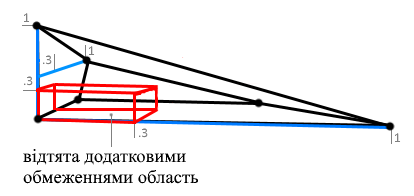
\includegraphics[width=0.6\textwidth]{figures/bounds}
  \caption{Графік функцій обмежень}
  \label{fig:bounds}
\end{figure}

Результати розрахунків для 3 різних наборів значень вагових коефіцієнтів $\vec{p} = (0.8, 0.1, 0.1)$, $\vec{p} = (0.05, 0.6, 0.35)$ та $\vec{p} = (0.333, 0.333, 0.334)$ були занесені до таблиці~\ref{tab:result}.

    \begin{landscape}% Landscape page
        \begin{table}[H]        
    	    \caption{Результати розрахунків}
	        \label{tab:result}
	        \footnotesize
        \begin{tabular}{c c c|c c c|c c c|c c c|c c c|c}
        	% head
        	% p
            $p_1$   & $p_2$   & $p_3$ 
        	% x
            & $x_1^*$ & $x_2^*$ & $x_3^*$
        	% fx
            & $f_1(\vec{x^*})$ & $f_2(\vec{x^*})$ & $f_3(\vec{x^*})$
        	% wx
            & $\omega(\vec{x^*})$ & $\omega(\vec{x^*})$ & $\omega(\vec{x^*})$
        	% pwx
            & $p_1\omega(\vec{x^*})$ & $p_2\omega(\vec{x^*})$ & $p_3\omega(\vec{x^*})$
        	% fx
            & $k_0$ \\
            \hline

            $0.8$ & $0.1$ & $0.1$ & $3.53571$ & $0.17857$ & $0.28571$ & $3.53571$ & $0.17857$ & $0.28571$ & $0.11607$ & $0.92857$ & $0.92857$ & $0.09285$ & $0.09285$ & $0.09285$ & $0.09285$ \\
            $0.1$ & $0.8$ & $0.1$ & $0.87218$ & $2.25563$ & $0.87218$ & $0.87218$ & $2.25563$ & $0.87218$ & $0.78195$ & $0.09774$ & $0.78195$ & $0.07819$ & $0.07819$ & $0.07819$ & $0.07819$ \\
			$0.1$ & $0.1$ & $0.8$ & $0.28571$ & $0.17857$ & $3.53571$ & $0.28571$ & $0.17857$ & $3.53571$ & $0.92857$ & $0.92857$ & $0.11607$ & $0.09285$ & $0.09285$ & $0.09285$ & $0.09285$ \\
			$0.05$ & $0.6$ & $0.35$ & $0$ & $1.83206$ & $2.16793$ & $0$ & $1.83206$ & $2.16793$ & $1$ & $0.26717$ & $0.45801$ & $0.05$ & $0.16030$ & $0.16030$ & $0.16030$ \\
			$0.6$ & $0.05$ & $0.35$ & $2.52631$ & $0$ & $1.47368$ & $2.52631$ & $0$ & $1.47368$ & $0.36842$ & $1$ & $0.63157$ & $0.22105$ & $0.05$ & $0.22105$ & $0.22105$ \\
			$0.6$ & $0.35$ & $0.05$ & $2.79310$ & $1.20689$ & $0$ & $2.79310$ & $1.20689$ & $0$ & $0.30172$ & $0.51724$ & $1$ & $0.18103$ & $0.18103$ & $0.05$ & $0.18103$ \\
			$0.05$ & $0.35$ & $0.6$ & $0$ & $1.20689$ & $2.79310$ & $0$ & $1.20689$ & $2.79310$ & $1$ & $0.51724$ & $0.30172$ & $0.05$ & $0.18103$ & $0.18103$ & $0.18103$ \\ 
			$0.35$ & $0.05$ & $0.6$ & $1.47368$ & $0$ & $2.52631$ & $1.47368$ & $0$ & $2.52631$ & $0.63157$ & $1$ & $0.36842$ & $0.22105$ & $0.05$ & $0.22105$ & $0.22105$ \\ 
			$0.35$ & $0.6$ & $0.05$ & $2.16793$ & $1.83206$ & $0$ & $2.16793$ & $1.83206$ & $0$ & $0.45801$ & $0.26717$ & $1$ & $0.16030$ & $0.16030$ & $0.05$ & $0.16030$ \\
			$0.333$ & $0.333$ & $0.334$ & $1.52098$ & $0.9506$ & $1.52840$ & $1.52098$ & $0.9506$ & $1.52840$ & $0.61975$ & $0.61975$ & $0.61789$ & $0.20637$ & $0.20637$ & $0.20637$ & $0.20637$ \\ 
        \end{tabular}
        \end{table}
        \begin{description}
        	\item[де] $\vec{x^*}$ --- ефективна альтернатива.
        \end{description}
    \end{landscape}

\subsection{Висновки}
В ході виконання лабораторної роботи було вивчено загальні положення методу обмежень. Було виконано приведення вихідних критеріїв задачі до безрозмірного вигляду та була розв’язана система нерівностей при мінімальному значенні параметра $k_0$.

Обчислення виконувались з різноманітними значеннями вектору вагових коефіцієнтів. Було визначено, що не усі варіанти пріоритету дозволяють досягнути компромісу, а лише дають рішення, що задовольняє обмеження задачі. Обираючи тип нерівності, ми можемо вести пошук тільки компромісного рішення, або, у разі його відсутності, отримати лише задовільне рішення.

\end{document}
